\chapter{Introduction} %fazer virar uma introduction
\label{chapter:intro}

Designing a game involves a conjunction of many different disciplines, for example: art, animation, sound, story, character creation, etc. Although the term game design is widely used in the industry to refer only to the design of the gameplay aspect, all the separate parts of design must properly work together in order to provide the player with a good experience \cite{zubek:2020}.

In this chapter we are going to present the necessary background information in order to understand what motivated this work. First, we will discuss the concept of game design and how it evolved through the ages. Then we will present some information about the game industry and the costs of developing a game. Lastly we will explain what procedural content generation (PCG) is and show a division of categories to better understand it.

After the motivation of the work is explained, we will present our objectives and preface the content of the next chapters. 

\section{Game design}

The importance of game design has increased throughout video game history. Designers of early games like Pong, shown here on Figure \ref{fig:pong}, or Spacewar! had very limited computing resources to work with, therefore it makes sense that they are simple and straightforward. Such games had little to no audio output, very primitive graphics and simple gameplay, sometimes borrowing ideas from well-established games, such as Pong, which is an electronic version of the Tabletennis sport \cite{wolf:2007}.

\begin{figure}[h]
    \caption{Atari's PONG arcade released in 1972}
    \centerline{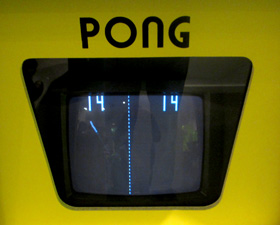
\includegraphics{images/introduction/PongScreenAtariOriginal.jpeg}}
    \legend{Source: \cite{pongmuseum:2021}}
    \label{fig:pong}
\end{figure}

In time, the technological advances made possible for more complex games to be created. Designing a game became much more nuanced and time consuming. 

\subsection{Evolution of the video game industry}

In 2020, the video game industry was already bigger than the movie industry and North American sports combined. The gaming industry has also experienced a big growth thanks to the COVID-19 pandemic \cite{marketwatch:2019}, since players are having more time at home for their hobby. But even before the pandemic, the industry was already in fast-grow along the last decades, as shown in Figure \ref{fig:growth_graph}.

\begin{figure}[h]
    \caption{Video game industry revenue through the ages}
    \centerline{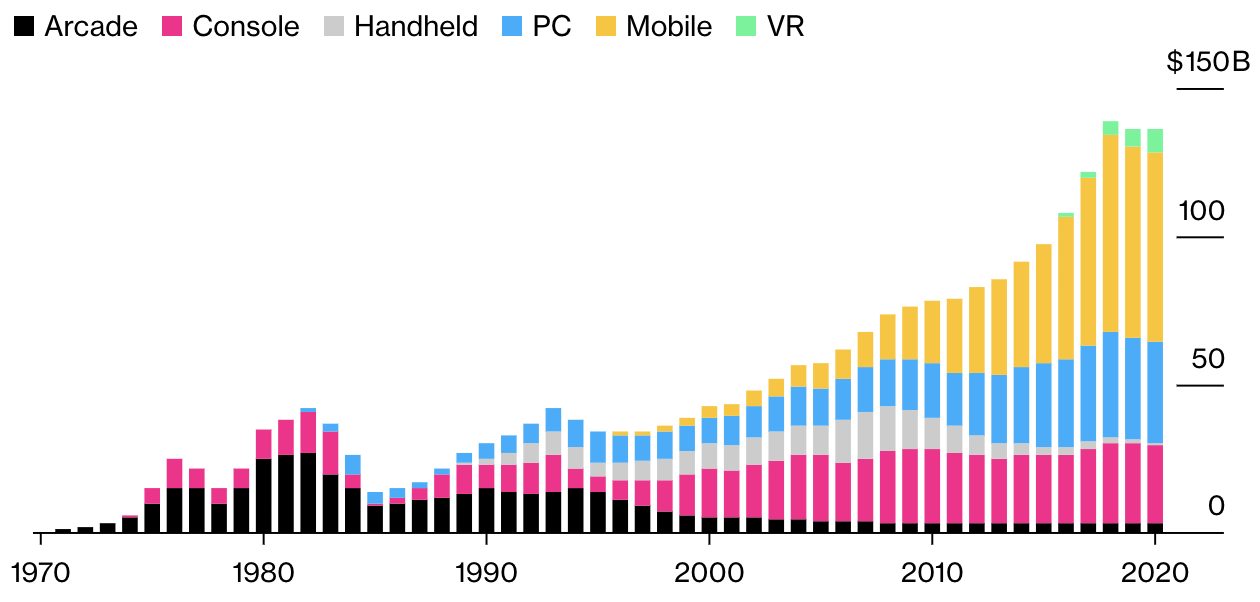
\includegraphics[width=13cm]{images/introduction/industry_growth.png}}
    \legend{Source: \cite{bloomberg:2019}}
    \label{fig:growth_graph}
\end{figure}

On the other hand, the cost of making games has increased dramatically as well. The cost of making Final Fantasy 7 remake, which was released in April 2020, for example, was roughly \$200 million, around \$120 million more than the original Final Fantasy 7, which was released in January 1997 \cite{cbr:2021}.

Triple-A games, which are games that are produced by mid-sized or major publishers \cite{steinberg:2007}, currently require the work of hundreds of people over the period of years to develop a single game. This is resulting in games not being as profitable for some developers, as few companies can afford developing long, diverse and polished games \cite{shaker:2016}.

One of the methods to reduce the cost of game designing is Procedural Content Generation (PCG), which uses algorithms to generate automatic content for the game.

\section{Procedural content generation}
\label{sec:pcg}

In the context of video games, PCG is defined as "the algorithmic creation of game content with
limited or indirect user input" \cite{togelius:2011}. In other words, PCG refers to software that is able to create game content by itself.

According to \textcite{doull:2008} there are 7 categories of PCG in games:

\begin{itemize}
\item \textbf{Runtime random level generation}: the generation of game levels while the game is being played. This is what people often think of when PCG in games is mentioned. In this category, an algorithm is responsible for generating random or pseudo-random levels for the game.

\item \textbf{Design of level content}: in this method, the automatically generated content is used at the level design stage to supplement human design skills. An algorithm can, for example, populate an environment created by the designer rapidly. Or the designer may choose specific generated levels to expand on.

\item \textbf{Dynamic world generation}: This technique is used to dynamically grow the environment that the player interacts on by using random seeds. In this case, the generated maps are never held in memory except as temporary structures to display.

\item \textbf{Instancing of in game entities}: in order to reach a statistically insignificant chance of repetition, in-game entities, such as like monsters, items, non-playable characters (NPCs), have some of their properties procedurally generated. These properties may be, for example, the position of the entity, its size, structure, etc.

\item \textbf{User mediated content}: this is a type of procedural generation where the user is in control. The technique offers a range of possibilities to users, who are responsible for putting them together in order to generate content.

\item \textbf{Dynamic systems}: some real-world systems such as group or weather behavior can be modelled using PCG techniques. This is widely used in combination of artificial intelligence (AI) in order to, for example, make NPCs react differently according to certain weather conditions.

\item \textbf{Procedural puzzles and plot generation}: this category is about using PCG in order to generate individual puzzle elements to increase replayability, e.g. changing door codes. Games that have its plot generated by PCG are also included in this category.
\end{itemize}

An example of a commercial game that was developed utilizing different PCG techniques is Electronic Arts's Spore. In this game, the player's objective is to evolve its own species, starting all the way from a microscopic organism until interstellar exploration. Entities on the game are generated by other players using in-game editors, which is an example of user mediated content generation. Worlds and galaxies are created through a combination of dynamic world generation and runtime random level generation. Moreover, some of the character animations are created procedurally \cite{wright:2007}. Figure \ref{fig:spore} shows user-generated characters standing on a procedurally generated world.

\begin{figure}[h]
    \caption{Screenshot of Spore gameplay}
    \centerline{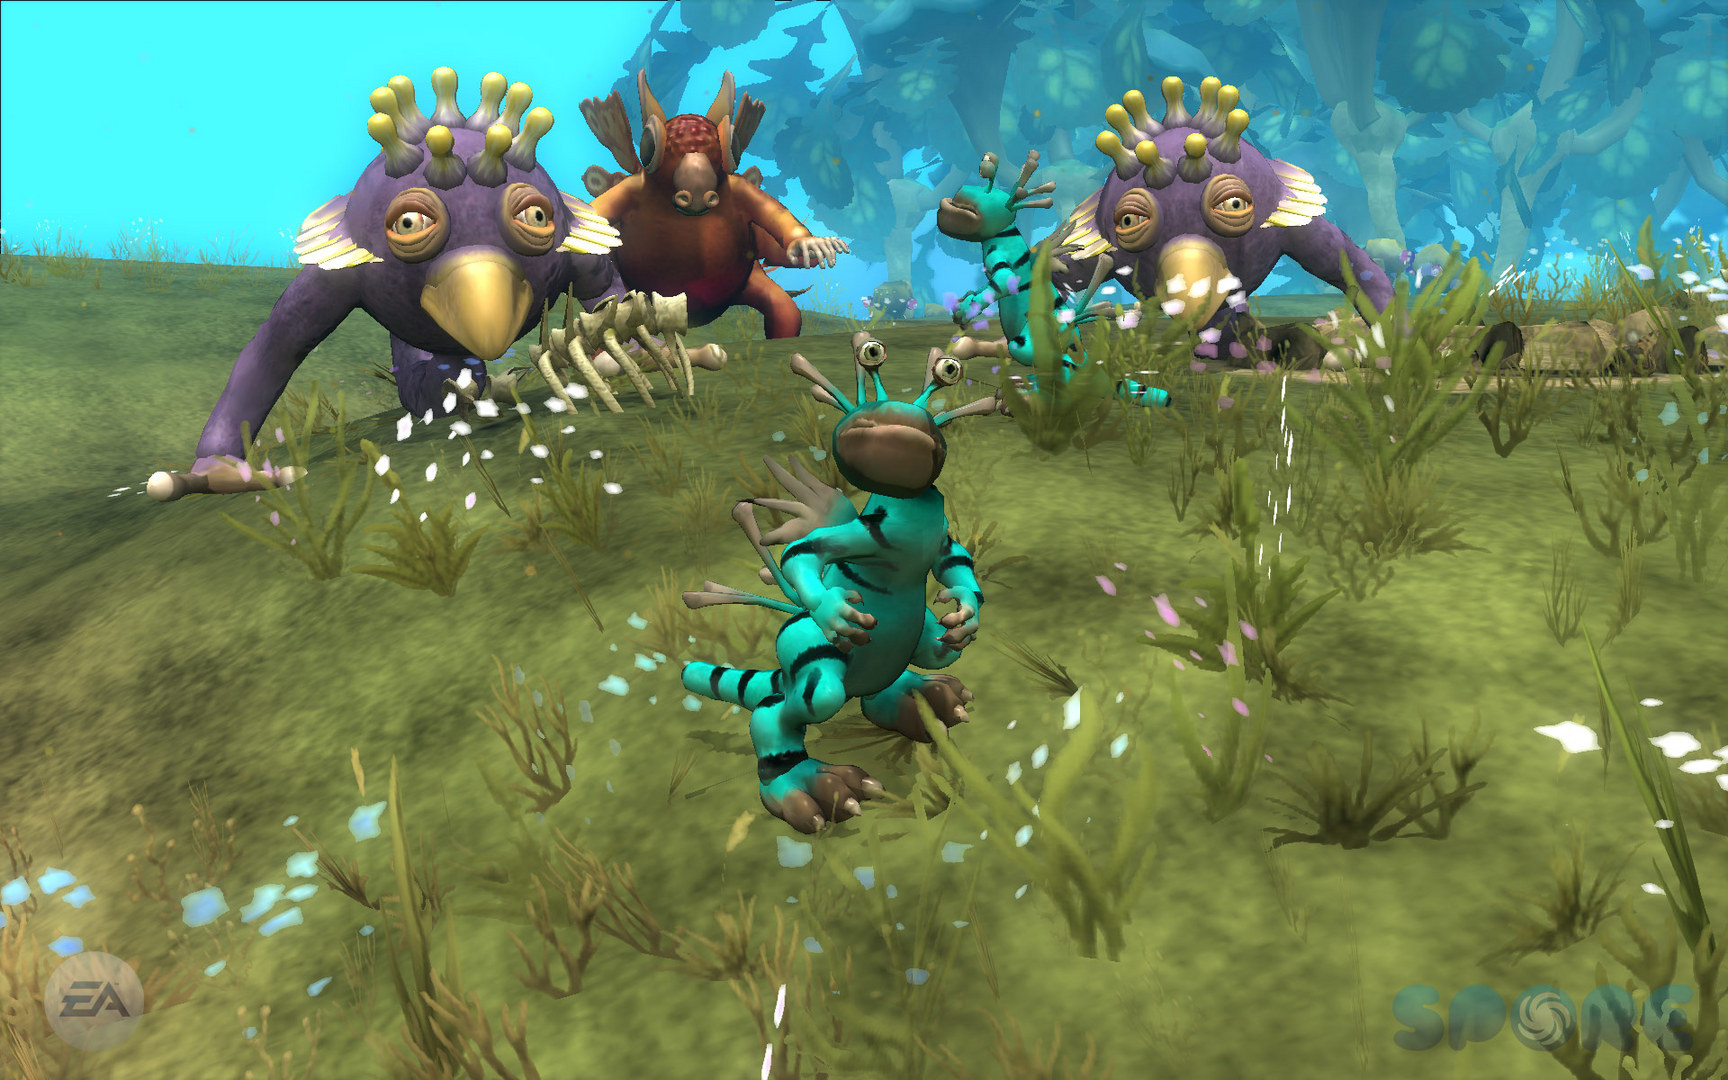
\includegraphics[width=13cm]{images/introduction/spore.jpg}}
    \legend{Source: \cite{ea:2008}}
    \label{fig:spore}
\end{figure}


\section{Dungeons in games}

One of the most notable applications of PCG in games is the creation of procedurally generated dungeons. A dungeon is a labyrinthic environment that the player can explore, as well as collect items, slay monsters, fall into traps, etc. Although originally the term "dungeon" refers to a labyrinth of prison cells, nowadays, there are dungeons representing caverns, castles, forests, underwater environments, etc \cite{shaker:2016}. 

This current definition of a dungeon can be probably tracked to the Dungeons and Dragons game, which is a tabletop Role-Playing Game (RPG) that had a huge influence in the development of video games throughout history. In fact, a specific type of computer RPG has spawned from the idea of exploring randomly generated dungeons: the roguelike genre. The name "roguelike" comes from the 1980's game Rogue, which featured procedurally generated dungeons that the player had to explore in search of an amulet \cite{brewer:2016}. A screenshot of a typical Rogue session can be seen in Figure \ref{fig:rogue}.

\begin{figure}[h]
    \caption{Screenshot of Rogue gameplay}
    \centerline{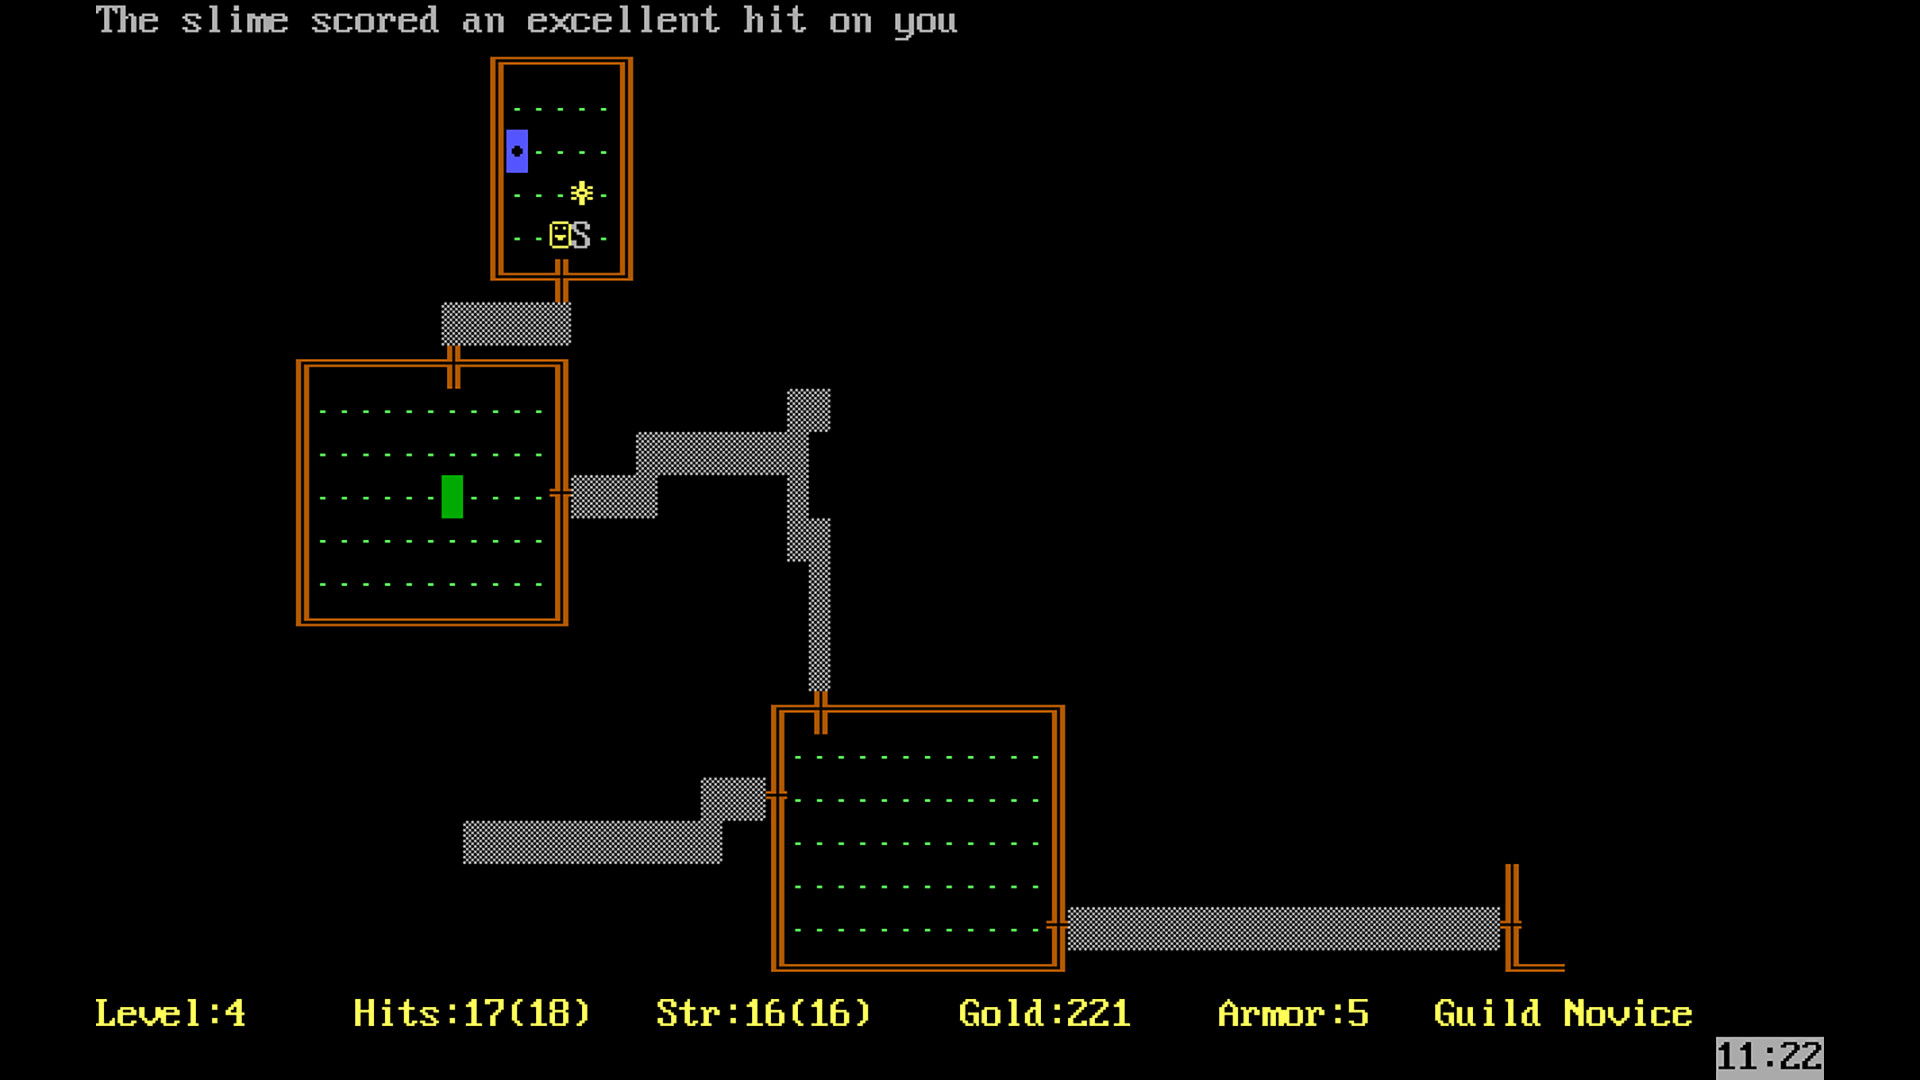
\includegraphics[width=13cm]{images/introduction/rogue.jpg}}
    \legend{Source: \cite{epyx:1985}}
    \label{fig:rogue}
\end{figure}

In \textcite{melan:2006} it is suggested that the design of the dungeon structure is very important to the creation of a good dungeon map. According to the author, a good map design is one that embodies the factors that make playing on a dungeon fun: exploration, decision making, consistent pace of action, discovery of secrets. Four different basic forms of dungeon maps, created from the author experience with RPG, were presented in \textcite{melan:2006},  shown here on Figure \ref{fig:basic_dungeons}. 

\begin{figure}[h]
    \caption{Basic dungeon structures}
    \centerline{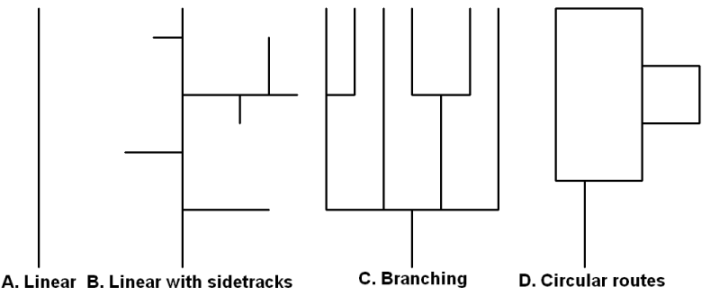
\includegraphics[width=13cm]{images/introduction/basic_dungeon.png}}
    \legend{Source: \cite{melan:2006}}
    \label{fig:basic_dungeons}
\end{figure}



\section{Objectives}
\label{sec:objectives}

Taking motivation from the information presented in the previous sections, this work has been elaborated with the objective of creating a PCG system to design cave-like dungeon maps for 2D top-down games.

More specifically, we will:

\begin{itemize}
\item \textbf{} Generate varied and cave-like dungeon maps from the combination of different algorithms.

\item \textbf{} Contribute to the PCG category of 'design of level content' by generating levels that can serve as a blueprint for game designers to build upon on the future.

\item \textbf{} Provide maps based on a set of criteria found in bibliography for what is considered a good dungeon map.

\item \textbf{} Evaluate if the generated maps match the criteria through a survey applied to video-game players.

\end{itemize}

\section{Organization of this work}

Next, on Chapter \ref{chapter:related}, we will cover works that are related to this one. After that, on Chapter \ref{chapter:proposal} our proposal will be expanded on and some background information will be provided in order to fully understand it. Following that, on chapter \ref{chapter:dev} we will provide details on our development and implementation. Chapter \ref{chapter:survey} will cover the creation of the survey and its results. Lastly on Chapter \ref{chapter:conclusion} we will discuss the conclusions of our work.

